\documentclass[12pt, a4paper]{article}

\usepackage[utf8]{inputenc}
\usepackage[ngerman]{babel}
\usepackage{amsmath, amssymb}
\usepackage[left=2.5cm, right=2.5cm, top=2.5cm, bottom=2.5cm]{geometry}
\usepackage{graphicx}
\usepackage{fancyhdr}
\usepackage{titling}
\usepackage{caption}
\usepackage{subcaption}
\usepackage{setspace}
\usepackage{footmisc}
\usepackage[colorlinks=false, pdfborder={0 0 0}]{hyperref}
\usepackage[font=footnotesize,labelfont=bf]{caption}
\usepackage[format=plain, indention=2em]{caption}
\graphicspath{{Image Sources/}}

\newcommand{\subtitle}[1]{%
	\posttitle{%
		\par\end{center}
	\begin{center}\large#1\end{center}
	\vskip0.5em}%
	}
	
	\addto\captionsngerman{\renewcommand{\figurename}{Fig.}}
	\onehalfspacing
	\renewcommand{\subsectionmark}[1]{}
	\renewcommand{\footnotelayout}{\setstretch{1.0}\footnotesize}
	\renewcommand{\labelenumi}{\Roman{enumi}}
	\renewcommand{\labelenumii}{\Roman{enumi}.\roman{enumii}}
	\renewcommand{\labelenumiii}{\Roman{enumi}.\roman{enumii}.\roman{enumiii}}
	\renewcommand{\labelenumiv}{\Roman{enumi}.\roman{enumii}.\roman{enumiii}.\roman{enumiv}}
	
	
	
	\title{W-Seminar}
	\subtitle{Deckblatt siehe ByCs}
	\author{Armin Binder }
	\date{SJ 2024/25}
	
	\begin{document}
\pagestyle{fancy}
\fancyhf{} 
\fancyfoot[C]{\thepage}

%\pagenumbering{arabic}
%	\fancyhf{}
%	\fancyfoot[R]{\thepage}
\maketitle
\thispagestyle{empty}
\pagebreak

\tableofcontents
\thispagestyle{empty}
\pagebreak

\section{Abstract}


\section{Einleitung}
\subsection{Geschichte und Bedeutung von Magnetfeldern und ihrer Messung}

%alternative: Geschichte und Bedeutung von Magnetfeldern
Magnetfelder und ihre Wechselwirkungen mit anderen natürlichen Effekten faszinieren den Menschen schon seit Jahrtausenden. Ihre Bedeutung - genau wie diejenige ihrer Bemessung - für das Leben auf der Erde ist kaum zu überschätzen. \paragraph{}
Der früheste Zeitpunkt, zu dem sich das geomagnetische Feld verlässlich datieren lässt liegt vor etwa 4,2 Milliarden Jahren im Hadaikum. Dies ist dementsprechend nach aktuellem Forschungsstand auch der früheste Zeitpunkt, ab den eine magnetosphärische Abschirmung der Erde vor kosmischer Strahlung angenommen werden kann\cite{tarduno25}. \newline
Wie man sich diese Abschirmung der Erde ungefähr vorstellen kann, sieht man in Fig. 1. \newline
\begin{figure}[h]
	\centering
	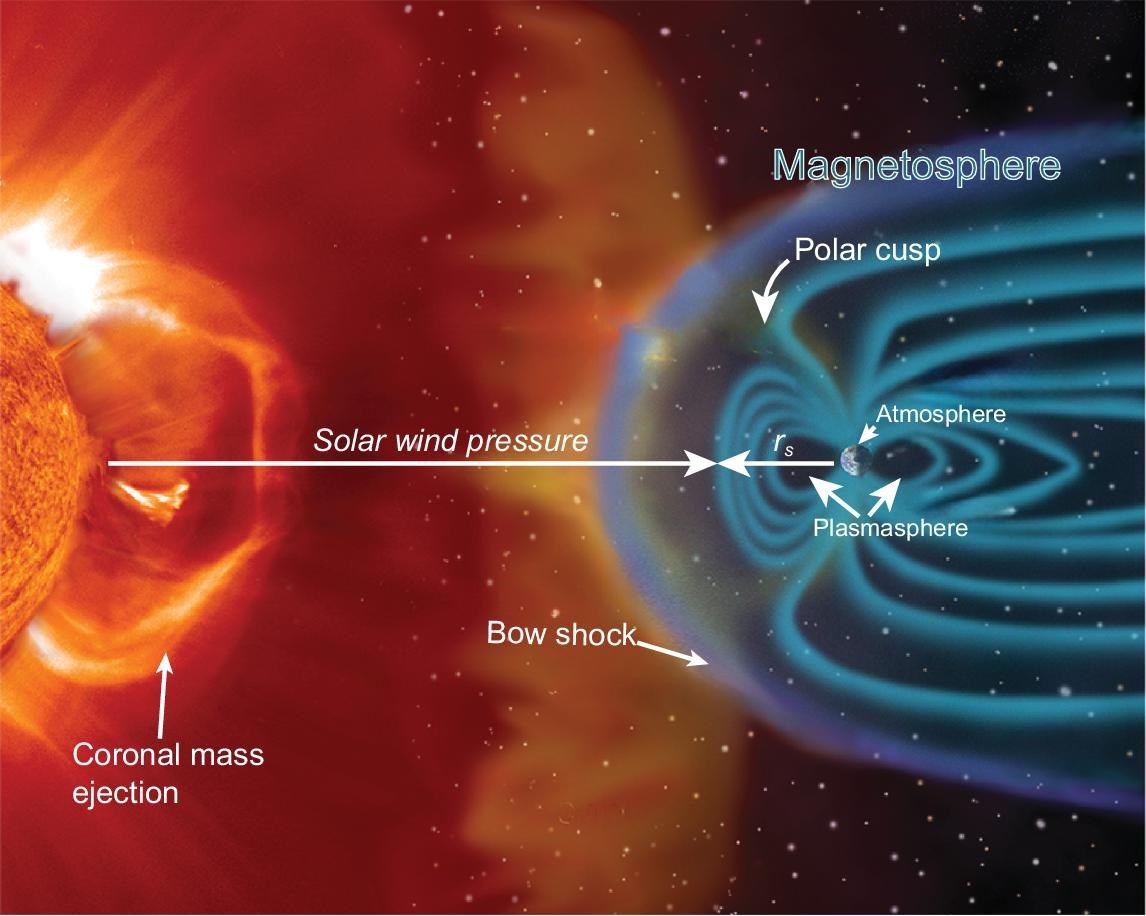
\includegraphics[height=8cm]{Fig1}
	\caption{Wesentliche Interaktionen der Sonne mit der Erde und ihrem Magnetfeld}
	\label{fig:1}
\end{figure}\newline
Auf diese Zeit lässt sich, durch genetische Studien bestimmt, auch eine erste nennenswerte Lebensform datieren, die man als "Last Universal Common Ancestor" bezeichnet. Es ist davon auszugehen, dass die magnetosphärische Abschirmung der Erde diese frühen Formen der Lebensbildung deutlich vereinfachte, da so möglicherweise auch viele andere Umgebungen außer metertiefem Wasser für Entwicklung von Leben in Frage kamen\cite{tarduno25}.\newline
Es gibt aber auch Hypothesen, nach denen zwar die magnetosphärische Abschirmung der Erde relevant für Weiterentwicklung von Leben war, der eigentliche Anstoß dieser Entwicklung aber durch die hohe Energie kosmischer Strahlung, die vor entstehen der Magnetosphäre ungebremst auf die Erde traf, stattfand\cite{tarduno25}.\newline
Paläomagnetische Daten zeigen einen starken Einbruch der Intensität des Erdmagnetfelds zu Zeiten gegen Ende des Ediacariums vor etwa 540 Millionen Jahren. Diese Zeit eines ultra-schwachen Erdmagnetfeldes impliziert eine wesentliche Erhöhung der Sauerstoffkonzentration in der Erdatmospähre, da hier immer größere Lebensformen existieren konnten. Diese erhöhte Konzentration lässt sich durch wieder verstärkten Einfluss kosmischer Strahlung adequat erklären\cite{tarduno25}.\newline
Zusammenfassend kann gesagt werden, dass die starken Fluktuationen im Erdmagnetfeld seit Enstehung dieses wie in Fig. 2 abgebildet jeweils erheblichen Einfluss auf die Entwicklung von Leben wie es jetzt besteht hatten.\newline
\begin{figure}[h]
	\centering
	
\includegraphics[height=10cm]{Fig2}
	\caption{Paläointensität als Indikator für wichtige Entwicklungen im Erdinneren, an der Erdoberfläche und in der Magnetosphäre, welche Einfluss auf Leben und Bewohnbarkeit der Erde haben. Paleointensitätshistorie von noch vorhandenen Steinen mit Einschränkungen durch Zirkon-Paläomagnetismus}
	\label{fig:2}
\end{figure}\paragraph{}

Wie diese kurze Zusammenfassung der Geschichte des Erdmagnetfeldes und seines Einflusses auf die Entwicklung von Leben zeigt, sind also Magneten und Magnetfelder Phänomene, mit denen die Menschheit seit jeher eng verbunden ist.\paragraph{}

Die frühesten Aufzeichnungen vom menschlichen Kontakt mit magnetischen Effekten stammen aus dem antiken China, ungefähr 4000 Jahre vor Christus. Hier wurden nach \cite{yang87} bereits Magnetsteine und magnetische Kompasse zur Navigation verwendet.\newline
Ausführlichere Aufzeichnungen existieren ungefähr ab dem 6. Jahrhundert vor Christus, zum Beispiel aus Griechenland und Indien\cite{singh19}. So versuchte sich der Naturphilosoph Thales von Milet als einer der ersten daran, die Anziehung von Eisen durch natürlich vorkommende Magnetsteine zu erklären, indem er ihnen eine Seelenkraft zusprach\cite{metioui22}.\newline
Währenddessen nutzte der indische Arzt Sushruta (ca. 6. Jahrhundert v.Chr.) Magnetsteine unter anderem als Chirurgiewerkzeug, um, unter anderem, Metallsplitter aus Wunden auf dem Schlachtfeld verletzter Soldaten zu entfernen\cite{singh19}.\newline 
Der ebenfalls griechische Philosoph Empedokles von Agrigent (ca. 5. Jahrhundert v.Chr.) versuchte sich an einer Erklärung magnetischer Phänomene mit Hilfe von Demokrits und Leukipps Atomtheorie, während Plutarch (ca. 1. Jahrhundert n.Chr.) von einer unsichtbaren Ausströmung, dem Duft eines Gegenstandes ähnlich, ausging, der für die magnetischen Anziehungskräfte verantwortlich war\cite{metioui22}.\paragraph{}

Über die nächsten Jahrhunderte dann gab es sehr viele pseudowissenschaftliche Ansätze die versuchten, Magnetismus zu erklären oder ihm fälschlicherweise Eigenschaften wie einen positiven Einfluss auf die Gesundheit zuzuschreiben. Trotzdem entwickelten sich parallel zum Beispiel auch in China die ersten magnetischen Nadelkompasse, um Navigation weiter zu vereinfachen\cite{metioui22}.\newline
Der erste tatsächlich wissenschaftliche Durchbruch beim Magnetismus gelang Peter Peregrinus de Maricourt 1269, als er in einem seiner Briefe über Magneten das Prinzip des magnetischen Dipols in Magnetsteinen beschrieb. Des weiteren beschrieb er auch die Grundlegenden Polgesetze und beobachtete, dass er durch zerkleinern der Steine keinen magnetischen Monopol schaffen konnte\cite{metioui22}.\newline
Robert Norman entdeckte um 1581 dann die magnetische Inklination. Er bemerkte, dass Kompassnadeln sich ohne Gegengewicht immer nach unten neigt, Richtung Norden. Er baute einen speziellen Kompass um diesen Effekt genauer zu messen und aus seinen Beobachtungen ließ sich folgern, dass die Ausrichtung einer Kompassnadel nicht auf die Orientierung zu einem festen Punkt zurückzuführen ist, sondern auf die am Erdmagnetfeld\cite{metioui22}.\newline
In seinem 1600 veröffentlichten Buch "De Magnete" fasste dann der englische Arzt und Naturphilosoph William Gilbert all seine Erkenntnisse zu Magnetismus und statischer Elektrizität zusammen, wobei hier seine klare Differenzierung dieser beiden Begriffe hervorzuheben ist. Neben der Feststellung, dass magnetische Eigenschaften Temperaturabhängig sind, stellte er fest, dass die Erde selbst eine Art riesiger Magnet mit zwei Polen ist und sich die Nadeln von Kompassen durch diese Magnetisierung der Erde ausrichteten\cite{singh19}.\paragraph{}

Im 18. Jahrhundert verdichteten sich dann Forschungsergebnisse zum Thema Magnetismus. Charles-Augustin de Coulomb entdeckte, dass die Anziehungskraft zweier magnetischer Körper zueinander umgekehrt proportional zum Quadrat des Abstands beider Körper ist\cite{metioui22}.\newline
Die führende Theorie zur Begründung magnetischer Effekte war die "{Effluvien Theorie}". Hier wurde davon ausgegangen, das eine unsichtbare Flüssigkeit magnetische und elektrische Effekte von einem Ort zum anderen überträgt\cite{singh19}.\newline
Später formulierten Carl Friedrich Gauss und Simeon Denis Poisson Coulombs Beobachtungen und Forschungsergebnisse als mathematische Gleichungen. Anfang des 19. Jahrhunderts dann entdeckte Christian Œrsted, dass elektrischer Strom magnetische Felder erzeugt. Diese Idee entwickelte Marie-André Ampère weiter und stellte die Theorie auf, dass die magnetische Kraft um ein Kabel einen kreisförmigen Charakter hat. Er lieferte auch als erster einen noch heute ansatzweise richtigen Erklärungsansatz für das Phänomen des Ferromagnetismus\cite{singh19}.\newline 
Michael Faraday entdeckte schließlich das Prinzip der magnetischen Induktion, welche nicht nur damals eine technologische Revolution anstieß\cite{singh19} sondern auch heute noch Verwendung in sehr vielen Bereichen unseres Lebens findet.\newline 
James Clerk Maxwell formulierte Faradays Konzepte, zusammen mit denen von unter anderem Ampère, schließlich in mathematischer Weise\cite{singh19}, heute bekannt als Maxwell-Gleichungen.\newline 
Ab dem späten 19. Jahrhundert dann arbeiteten Forscher wie Pierre Curie, Paul Langevin und Pierre Weiss daran, mögliche Erklärungen für magnetische Effekte und den Einfluss von Umweltvariablen wie Temperatur auf diese zu etablieren, die aber alle nur bedingt erfolgreich blieben\cite{singh19}.\paragraph{}

Nach Einführung der neuen Prinzipien der Quantenmechanik durch unter anderem Heisenberg, Born, Schroedinger und Dirac in den 1920er Jahren gelang dann aber endlich mehr und mehr, Magnetismus und seine Ursprünge zu erklären.\newline
Physiker wie John Hasbrouck Van Vleck, Yakov Grigor’evich Dorfman, Wolfgang Pauli, Werner Heisenberg und Lew Dawidowitsch Landau erarbeiten über viele Jahre, größtenteils basierend auf den alten Ansätzen von Langevin, Curie und Weiss die bis heute noch gültigen Erklärungen der meisten magnetischen Phänomene auf Quantenebene, die nur in wenigen Ausnahmefällen (wie zum Beispiel Quantum Spin Liquids\footnote{Seltene magnetische Zustände, bei denen sich Elektronenspins selbst bei extrem niedrigen Temperaturen nie in einen festen Muster ordnen und starke Quantenfluktuationen zeigen}) nicht vollständig anwendbar sind\cite{singh19}.\newline 





\subsection{Magnetfeldmessungen und der Hall-Effekt}
Über diese lange Geschichte der Magnetfeldforschung wurden auch dementsprechend viele verschiedene Methoden entwickelt um Magnetfelder zu messen, die von sehr einfachen Methoden bis hin zu hochkomplexen Quantenmethoden reichen. Hier eine kurze Zusammenfassung einiger relevanter Messmethoden:
\begin{itemize}
	\item \textbf{Magnetresonanzmessungen:} Wasser, entweder als kleine Probe oder fließend durch eine kleine Röhre, wird in einer Anregungsspule von Radiowellen angeregt. Das magnetische Moment der Wassernukleonen, beeinflusst durch ein externes Magnetfeld, wird entweder über nukleare Induktion\footnote{Induktionseffekte, die durch das magnetische Moment von Nukleonen hervorgerufen werden} oder über Resonanzabsorption ausgelesen
	\item \textbf{Magnetische Flussmeter:} Durch Änderungen des Magnetfelds wird in einer Messspule eine Spannung induziert. Diese Spannung wird über die Zeit integriert, um den magnetischen Fluss zu bestimmen
	\item \textbf{Photoelektrische Flussmeter:} Durch ein Magnetfeld wird eine Bewegung erzeugt, die in ein Lichtsignal umgewandelt und von einem Photosensor gemessen wird, um den magnetischen Fluss zu bestimmen
	\item \textbf{Hall-Methode:} An einen kleinen Metall- oder Halbleiterstreifen wird eine Anregungsspannung angelegt. Wirkt ein Magnetfeld auf die bewegten Ladungsträger, werden diese durch die Lorentzkraft seitlich abgelenkt. Dadurch entsteht eine messbare Hall-Spannung quer zum Stromfluss, aus der die Stärke des Magnetfelds bestimmt werden kann
	\item \textbf{Fluxgate-Magnetometer:} Um einen ferromagnetischen Kern werden mindestens drei Spulen angebracht:
	\subitem - Eine Wechselstrom-Anregungsspule, die den Kern  alternierend sättigt 
	\subitem - Eine Messspule, an der im Idealfall immer eine Nullspannung anliegt
	\subitem - Eine Gleichstrom-Bias-Spule, die ein externes Magnetfeld ausgleicht, sodass die Messspule wieder Nullspannung ausliest
	\newline
	Aus der Höhe des Gleichstroms, der zur Neutralisierung des Feldes benötigt wird, lässt sich die Stärke des externen Magnetfelds bestimmen
	\item \textbf{Magneto-Resistenz-Messungen:}
	\item \textbf{Visuelle Magnetfeldkartierung:}
	\item \textbf{Teilchenstrahl-Beobachtung: }
	\item \textbf{Atomare Magnetometer:}
	\item \textbf{Spin-Exchange-Relaxationsfreies (SERF) Magnetometer:}
	\item \textbf{Optisch gepumptes Magnetometer (OPM):}
	\item \textbf{Supraleitende Quanteninterferenzgeräte:}
\end{itemize}


\subsection{Projektziel und thematischer Bezug}


\section{Funktionsweise der X-Hall-Architektur}
Im vorherigen Kapitel wurden bereits die grundlegende Funktionsweise von Hall-Sensoren sowie typische Architekturen solcher Systeme behandelt.\paragraph{}
Die für diese Arbeit gewählte Architektur, die sogenannte \textbf{X-Hall-Architektur} unterscheidet sich aber von den zuvor genannten Architekturen in mehreren relevanten Aspekten. Im Folgenden soll diese spezifische Architektur vorgestellt werden und auf ihre Vor- sowie Nachteile eingegangen werden, ebenso wie auf die Gründe zur Wahl genau dieser %genauen 
Architektur für diese Arbeit.

\subsection{Geschichte und Konzept}
Bei der X-Hall-Architektur handelt es sich um eine recht neue Form des Hall-Sensors. Erstmalig wurde sie gegen Ende des Jahres 2018 auf dem IMEKO\footnote{International Measurement Confederation} 
World Congress vorgestellt \textbf{\cite{cres19}}. \newline
Die Entwicklung dieser neuen Art Hall-Sensor wurde insbesondere durch den Bedarf für Magnetfeldsensoren mit immer größeren Frequenzbandbreiten vorangetrieben, die grundlegende Bestandteile unter anderem von Sicherheitsschaltungen vieler moderner Stromversorgungskreisläufe sind\textbf{\cite{cres18}\cite{cres19}\cite{cres20}\cite{cres21}}. Die bisher genutzten Sensortypen und Architekturen, wohlgemerkt nicht exklusiv Hall-Sensoren, wiesen aber bereits durch ihren Aufbau alle gewisse Einschränkungen und Probleme auf, die ihre Einsetzbarkeit limitierten\textbf{\cite{cres18}\cite{cres19}\cite{cres21}}. \newline
Ziel der neuen Sensorarchitektur sollte es also sein, alle Aspekte, die für so einen Magnetfeldsensor relevant sind, in sich zu vereinen\textbf{\cite{cres19}}: 
\begin{itemize}
	\item Sehr hohe bemessbare Frequenzbandbreiten von Magnetfeldern %Nochmal seperat bestätigen
	\item Fähigkeiten, Gleichspannung (indirekt) zu messen
	\item Mögliche CMOS\footnote{Complementary Metal-Oxide Semiconductor = komplementärer Metalloxid-Halbleiter}-Integration
	\item Galvanische Isolation\footnote{Elektrische funktionale Sektionen sind so voneinander isoliert, dass es keinen direkten Stromfluss zwischen ihnen gibt}
	\item Keine Wärmeabstrahlung
	\item Geringer Flächenbedarf %Kleines Profil
	\item Geringe Produktionskosten
\end{itemize} 
Ergebnis dieses Forschungsprojekts war die X-Hall-Architektur.\newline
Einfach gesagt handelt es sich hierbei um eine Hall-Sonde mit jeweils vier Vorspannungs\footnote{Strom der durch den Sensor fließt, um den Hall-Effekt erst zu ermöglichen}- und vier Auslesekontakten (was jeweils das doppelte der jeweiligen Kontaktarten bei typischen Hall-Sensoren ist), die an der aktiven Fläche des Sensors angebracht sind. Durch eine elektrische Verbindung jeweils zweier diagonal gegenüberliegender Auslesekontakte vor dem eigentlichen Auslesevorgang wird gewährleistet, dass mögliche Defekte und Offsetspannungen\footnote{Ungewollte Spannungen, die selbst dann gemessen werden können, wenn der theoretische Messwert 0 sein sollte} auf der größeren aktiven Fläche unter anderem durch so entstehende Mittelungseffekte kompensiert werden. Dies führt zu einer einer höheren Genauigkeit und Stabilität der Messwerte.

\subsection{Aufbau und Funktionsweise}
Bei der aktiven Fläche eines X-Hall-Sensors handelt es sich in der Regel um einen oktagonal geformten, sogenannten n-Well\footnote{n-dotierte ``Halbleitertasche'' innerhalb eines p-dotierten Substrats} \cite{cres18}. \newline
Die n-Dotierung der aktiven Sensorfläche wird aufgrund einer höheren strombezogenen Empfindlichkeit\footnote{Begründet durch höhere Elektronenmobilität in n-Typ-Halbleitern} im Gegensatz zu p-dotierten Halbleitern präferiert. %bevorzugt?
Auch ist die Umschließung des n-Wells mit einem p-dotierten Material zwar für die grundlegende Sensorfunktion nicht essenziell, %auf nichtverwendung in Arbeit aufgrund komplexität hinweisen? 
sollte jedoch  angestrebt werden, da nur so eine effektive elektrische Isolation gegenüber dem Substrat erreicht werden kann\cite{cres20}.\newline
Der Zugang zur aktiven Fläche erfolgt über insgesamt acht Kontakte, die sich in vier großflächige Vorspannungskontakte und vier möglichst kleine Auslesekontakte unterteilen lassen. Die Vorspannungskontakte profitieren aufgrund ihrer Größe von sehr niedrigen Widerständen beim Anlegen der Vorspannung, während die Auslesekontakte so klein wie möglich sein sollten, da so die möglichen Effekte parasitärer Kapazitäten\footnote{Unerwünschte Kapazität, die durch geringe physische Nähe zwischen elektrischen Bauteilen entsteht} % , ???
wie etwa Signalverzerrungen oder erhöhtes Rauschen des Signals minimiert werden können\cite{cres19}.\newline
An die in Fig.~\ref{fig:3}(a) als B und T bezeichneten Vorspannungskontakte werden nominal gleiche Vorspannungsströme ($I_A=I_B$) angelegt, während die als L und R bezeichneten Kontakte jeweils als Erdungskontakte dienen\cite{cres19}. Die Auslesekontakte sind von 1 bis 4 durchnummeriert.\newline
In der aktuellen Konfiguration kann die gesamte Sensorsonde in zwei innere Sensorsonden untergliedert werden, die in Fig.~\ref{fig:3}(a) als Probe A und Probe B bezeichnet sind. Dies ist eine direkte Folge aus der in Fig.~\ref{fig:3}(b) gezeigten Stromstärkeverteilung zwischen den Kontakten auf dem Halbleiter, da der Strom über die Erdung bereits abgeführt wird, bevor er die zweite innere Sonde erreichen kann\cite{cres20}.
\begin{figure}
	\centering
	%Fig. 1-a
	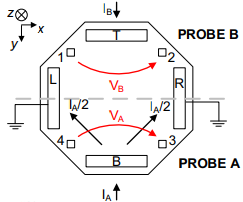
\includegraphics[height=5cm]{Fig3.1}	
	\hspace{0.5cm}
	%Fig. 1-b
	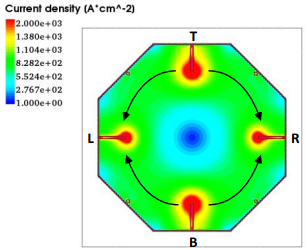
\includegraphics[height=5cm]{Fig3.2}
	\caption{(a) Skizze des Aufbaus der X-Hall-Sonde, (b) Stromstärkeverteilung auf der X-Hall-Sonde, basierend auf einer beispielhaften Vorstromstärke von $I_A=I_B=500\mu{A}$}
	\label{fig:3}
\end{figure}\newline
Diese inneren Sonden funktionieren, unabhängig voneinander, jeweils wie gewöhnliche stromverzweigende Hall-Sonden, bei denen die jeweilige Stromdichte $J_A$ oder $J_B$ in zwei gleiche Stromdichten $J_{A,L}$ und $J_{A,R}$ beziehungsweise $J_{B,L}$ und $J_{B,R}$ aufgespalten werden. Dementsprechend gilt für jeweiligen Potentiale zwischen den Messkontakten 1 und 2 beziehungsweise 3 und 4 in Abwesenheit eines Magnetfelds: $V_A=V_B=0$ \cite{cres21}.\newline
Liegt nun ein Magnetfeld $B_Z$ vor, entsteht aufgrund der Lorentzkräfte die auf die Ladungsträger wirken ein Ungleichgewicht im Stromfluss, was dazu führt, dass nun vereinfacht $V_A=V_\mathrm{Hall}$ und $V_B=-V_\mathrm{Hall}$ (Da der Stromfluss in der zweiten inneren Sonde in die entgegengesetzte Richtung des Stroms von Sonde A verläuft).\newline
In Realität lassen sich jedoch Asymmetrien in der Sensorstruktur, globale Inhomogenitäten von Materialien und andere Defekte nicht vermeiden, weshalb für die gemessenen Spannungen $V_A$ und $V_B$ tatsächlich gilt:
\begin{equation}
	V_A=V_\mathrm{H,Sonde}+V_\mathrm{OS}^{(A)}
	\label{eq:1}
\end{equation}
\begin{equation}
	V_B=-V_\mathrm{H,Sonde}+V_\mathrm{OS}^{(B)}
	\label{eq:2}
\end{equation}
$V_\mathrm{OS}^{(A)}$ und $V_\mathrm{OS}^{(B)}$ sind die Offsetspannungen der jeweiligen inneren Sonde\cite{cres20}.\newline
Da beide inneren Sonden sich nichtsdestotrotz die gleiche aktive Sensorfläche teilen, kann angenommen werden, dass das Vorzeichen von $V_\mathrm{OS}^{(A)}$ und $V_\mathrm{OS}^{(B)}$ identisch ist, auch wenn sich ihre jeweiligen Werte aufgrund lokaler Defekte unterscheiden können\cite{cres21}. Deshalb kann angenommen werden, dass die Hauptquelle der Offsets sehr wahrscheinlich für beide inneren Sonden die selbe ist\cite{cres20}.\newline
\begin{figure}
	\centering
	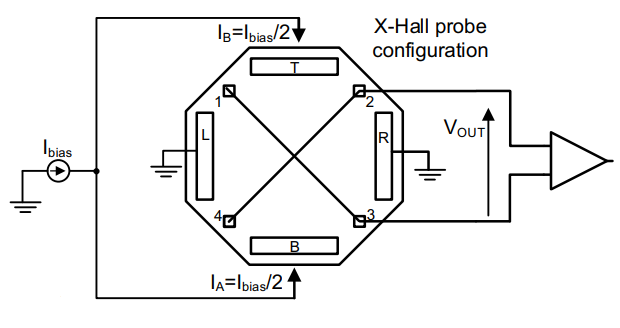
\includegraphics[height=5cm]{Fig4}
	\caption{Schematischer Schaltplan einer X-Hall-Sonde}
	\label{fig:4}
\end{figure}
Wie in Fig.~\ref{fig:4} gezeigt besteht die eigentliche und namensgebende Besonderheit der X-Hall-Architektur in einer Überkreuzverbindung der diagonal gegenüberliegenden Paare von Auslesekontakte (1 mit 3 und 2 mit 4). Daraus folgt:
\begin{equation}
	V_A=-V_B=V_\mathrm{H,Sonde}
	\label{eq:3}
\end{equation}
Unter der Annahme gleicher Vorzeichen beider Offsetspannungen und einer Substitution von (\ref{eq:1}) und (\ref{eq:2}) in (\ref{eq:3}) wird  impliziert:
\begin{equation}
	V_\mathrm{OS}^{(A)}=V_\mathrm{OS}^{(B)}=0
	\label{eq:4}
\end{equation}
Physikalisch gesehen erzeugt die Überkreuzverbindung der Auslesekontakte eine  Randbedingung in der aktiven Fläche, welche die Ladungsverteilung so beeinflusst, dass Offsetspannungen minimiert werden \cite{cres21}. 
Durch die Überkreuzverbindung sind beide Kontakte elektrisch verbunden, was dazu führt, dass sich die Ströme der beiden Kontakte gegenseitig ausbalancieren. %Dies ist Teil der typischen Ladungsverteilung hin zum energetisch günstigsten Zustand des Systems. 
Aufgrund dieser ladungsverschiebenden Effekte gleicht das System selbstständig ungewollte Offsets oder Defekte und damit verbundene energetisch ungünstige Ladungsverteilungen – ob lokal oder global – aus. %da das System bestrebt ist, seinen energetisch günstigen Zustand zu erreichen. 
So werden Anteile dieser ungünstigen Ladungsverteilungen in den tatsächlich ausgelesenen Messwerten minimiert.\newline
Trotzdem wird es immer vereinzelte lokale Defekte und Offsets geben, die zu einer verbleibenden Offsetspannung führen und jeweils zu $V_A$ und $V_B$ hinzugerechnet werden müssen. Die X-Hall-Architektur strebt also primär an, globale Defekte und Offsets mit starkem Einfluss auf Messergebnisse auszugleichen und nicht, diese vollständig zu eliminieren\cite{cres21}.

\subsection{Vorteile und Nachteile der Architektur}
\centering
Dieser Abschnitt wird in der vollständigen Arbeit weiter ausgeführt werden (Inhalt: Vor- und Nachteile der Architektur und evtl. eingehen auf diese als Gründe für die Wahl dieser spezifischen Sensorarchitektur)

\subsection{(Erwartete) Leistungscharakteristika der Architektur}


\section{Praktische Umsetzung des X-Hall-Sensors}
\subsection{Die Finite Element Methode}

\subsection{Entwicklung eines Sensor-Layouts}

\subsection{Praktische Implementierung des Sensors}


\section{Vergleich mit anderen Hall-Sensoren}
\subsection{Quantitativer Vergleich}

\subsection{Qualitativer Vergleich}	

\section{Fazit}





\section*{%Literaturverzeichnis%
}	%\clearpage
\newpage
\begin{thebibliography}{}
	\addcontentsline{toc}{section}{Literaturverzeichnis}
	
	\bibitem{tarduno25}
	\textbf{John A. Tarduno, Tinghong Zhou, Wentao Huang, Jaganmoy Jodder}, Earth’s magnetic field and its relationship to the origin of
	life, evolution and planetary habitability. National Science Review, vol. 12, issue 5, May 2025, doi.org/10.1093/nsr/nwaf082 
	
	\bibitem{singh19}
	\textbf{Navinder Singh, Arun M. Jayannavar}, A Brief history of mangnetism. Physical Research Laboratory Ahmedabad and IOP Bhubaneswar, India, 2019, arXiv:1903.07031v1 [physics.pop-ph]
	
	\bibitem{metioui22}
	\textbf{Abdeljalil Métioui}, Brief Historical Review about
	Magnetism: From the Ancient Greeks up the Beginning of the XXth Century. Journal of Biomedical Research and Environmental Sciences (J Biomed Res Environ Sci), doi: 10.37871/jbres1561
	
	\bibitem{yang87}
	\textbf{You-qing Yang}, Magnetic materials in china, in 3rd international conference on physics of magnetic materials (9-14 Sept. 1986). W. Gorzkowski, H. Lochowicz, and H. Szymczak Eds. World Scientific (1987). [so übernommen aus \cite{singh19}]
	
	
	
	
	
	\bibitem{henrichsen98}
	\textbf{K. N. Heinrichsen}, Overview of magnet measurement methods. CERN Accelerator School (CAS 97): Measurement and Alignment of Accelerator and Detector Magnets, Anacapri, Italy, April 1997, 127-141, 1997
	
	\bibitem{bai23}
	\textbf{Xuanyao Bai, Kailun Wen, Donghong Peng, Shuangqiang Liu, Le Luo}, Atomic magnetometers and their application in industry. Front. Phys., vol. 11, June 2023, doi: 10.3389/fphy.2023.1212368
	
	\bibitem{kiehl25}
	\textbf{Christopher Kiehl et al.}, Accurate vector optically pumped magnetometer with microwave-driven Rabi frequency measurements. Optica, vol. 12, no.1, pp. 77-87, Januar 2025, doi: 10.1364/OPTICA.542502
	
	\bibitem{Drung07}
	\textbf{D. Drung et al.}, Highly sensitive and easy-to-use SQUID sensors. IEEE Transactions on Applied Superconductivity, vol. 17, no. 2, pp. 699-704, June 2007, doi: 10.1109/TASC.2007.897403
	
	\bibitem{wikiSerf}
	\url{https://en.wikipedia.org/wiki/SERF}; Zugriff am 20.10.2025, 00:05 
	
	
	
	
	
	\bibitem{paun13}
	\textbf{Maria-Alexandra Paun, JM. Salesse, M. Kayal}, Hall Effect Sensors Design, Integration and Behavior Analysis. Journal of Sensors and Actuator Networks, 2013, 2, pp. 85-97, doi: 10.3390/jsan2010085
	
	\bibitem{cres18}
	\textbf{M. Crescenti et. al.}, Bandwith enhancement in Hall Probe by X-Hall DC biasing. XXII World Congress of International Measurement Confederation (IMEKO 2018), Journal of Physics: Conf. Series \textbf{1065} (2018) 052031, Belfast, United Kingdom, 2018, doi: 10.1088/1742-6596/1065/5/052031
	
	\bibitem{cres19}
	\textbf{M. Crescenti et. al.}, A  Broadband Current Sensor based on the X-Hall Architecture. 2019 26th IEEE International Congerence on Electronics, Circuits and Systems (ICECS), Genoa, Italy, 2019, pp. 807-810, doi: 10.1109/ICECS46596.2019.8964955
	
	\bibitem{cres20}
	\textbf{M. Crescenti et. al.}, Experimental Assessment of a Broadband Current Sensor based on the X-Hall Architecture. 2020 IEEE International Instrumentation and Measurement Technology Conference (I2MTC), Dubrovnik, Croatia, 2020, pp. 1-6, doi: 10.1109/I2MTC43012.2020.9128994
	
	\bibitem{cres21}
	\textbf{M. Crescenti et. al.}, The X-Hall Sensor: Towards Integrated Broadband Current Sensing. IEEE TRANSACTIONS ON INSTRUMENTATION AND MEASUREMENT, vol. 70, pp. 1-12, 2021, doi: 10.1109/TIM.2020.3036764
	
	
	
	
	
	
	
	
\end{thebibliography}

\section*{Grafikquellen}
\addcontentsline{toc}{section}{Grafikquellen}
\begin{description}
	\item \textbf{Fig. 1}: \url{https://www.esa.int/Science_Exploration/Human_and_Robotic_Exploration/Lessons_online/The_effects_of_magnetic_fields}; Zugriff am 19.10.2025, 20:34
	\item \textbf{Fig. 2}: Übernommen aus \cite{tarduno25}, Fig. 9
	\item \textbf{Fig. 3-a}: Übernommen aus \cite{cres18}, Fig. 1a
	\item \textbf{Fig. 3-b}: Übernommen aus \cite{cres20}, Fig. 2
	\item \textbf{Fig. 4}: Übernommen aus \cite{cres18}, Fig. 2a
	
\end{description}


\end{document}
